% Options for packages loaded elsewhere
\PassOptionsToPackage{unicode}{hyperref}
\PassOptionsToPackage{hyphens}{url}
\PassOptionsToPackage{dvipsnames,svgnames,x11names}{xcolor}
%
\documentclass[
  letterpaper,
  DIV=11,
  numbers=noendperiod]{scrartcl}

\usepackage{amsmath,amssymb}
\usepackage{iftex}
\ifPDFTeX
  \usepackage[T1]{fontenc}
  \usepackage[utf8]{inputenc}
  \usepackage{textcomp} % provide euro and other symbols
\else % if luatex or xetex
  \usepackage{unicode-math}
  \defaultfontfeatures{Scale=MatchLowercase}
  \defaultfontfeatures[\rmfamily]{Ligatures=TeX,Scale=1}
\fi
\usepackage{lmodern}
\ifPDFTeX\else  
    % xetex/luatex font selection
\fi
% Use upquote if available, for straight quotes in verbatim environments
\IfFileExists{upquote.sty}{\usepackage{upquote}}{}
\IfFileExists{microtype.sty}{% use microtype if available
  \usepackage[]{microtype}
  \UseMicrotypeSet[protrusion]{basicmath} % disable protrusion for tt fonts
}{}
\makeatletter
\@ifundefined{KOMAClassName}{% if non-KOMA class
  \IfFileExists{parskip.sty}{%
    \usepackage{parskip}
  }{% else
    \setlength{\parindent}{0pt}
    \setlength{\parskip}{6pt plus 2pt minus 1pt}}
}{% if KOMA class
  \KOMAoptions{parskip=half}}
\makeatother
\usepackage{xcolor}
\setlength{\emergencystretch}{3em} % prevent overfull lines
\setcounter{secnumdepth}{-\maxdimen} % remove section numbering
% Make \paragraph and \subparagraph free-standing
\makeatletter
\ifx\paragraph\undefined\else
  \let\oldparagraph\paragraph
  \renewcommand{\paragraph}{
    \@ifstar
      \xxxParagraphStar
      \xxxParagraphNoStar
  }
  \newcommand{\xxxParagraphStar}[1]{\oldparagraph*{#1}\mbox{}}
  \newcommand{\xxxParagraphNoStar}[1]{\oldparagraph{#1}\mbox{}}
\fi
\ifx\subparagraph\undefined\else
  \let\oldsubparagraph\subparagraph
  \renewcommand{\subparagraph}{
    \@ifstar
      \xxxSubParagraphStar
      \xxxSubParagraphNoStar
  }
  \newcommand{\xxxSubParagraphStar}[1]{\oldsubparagraph*{#1}\mbox{}}
  \newcommand{\xxxSubParagraphNoStar}[1]{\oldsubparagraph{#1}\mbox{}}
\fi
\makeatother


\providecommand{\tightlist}{%
  \setlength{\itemsep}{0pt}\setlength{\parskip}{0pt}}\usepackage{longtable,booktabs,array}
\usepackage{calc} % for calculating minipage widths
% Correct order of tables after \paragraph or \subparagraph
\usepackage{etoolbox}
\makeatletter
\patchcmd\longtable{\par}{\if@noskipsec\mbox{}\fi\par}{}{}
\makeatother
% Allow footnotes in longtable head/foot
\IfFileExists{footnotehyper.sty}{\usepackage{footnotehyper}}{\usepackage{footnote}}
\makesavenoteenv{longtable}
\usepackage{graphicx}
\makeatletter
\def\maxwidth{\ifdim\Gin@nat@width>\linewidth\linewidth\else\Gin@nat@width\fi}
\def\maxheight{\ifdim\Gin@nat@height>\textheight\textheight\else\Gin@nat@height\fi}
\makeatother
% Scale images if necessary, so that they will not overflow the page
% margins by default, and it is still possible to overwrite the defaults
% using explicit options in \includegraphics[width, height, ...]{}
\setkeys{Gin}{width=\maxwidth,height=\maxheight,keepaspectratio}
% Set default figure placement to htbp
\makeatletter
\def\fps@figure{htbp}
\makeatother
% definitions for citeproc citations
\NewDocumentCommand\citeproctext{}{}
\NewDocumentCommand\citeproc{mm}{%
  \begingroup\def\citeproctext{#2}\cite{#1}\endgroup}
\makeatletter
 % allow citations to break across lines
 \let\@cite@ofmt\@firstofone
 % avoid brackets around text for \cite:
 \def\@biblabel#1{}
 \def\@cite#1#2{{#1\if@tempswa , #2\fi}}
\makeatother
\newlength{\cslhangindent}
\setlength{\cslhangindent}{1.5em}
\newlength{\csllabelwidth}
\setlength{\csllabelwidth}{3em}
\newenvironment{CSLReferences}[2] % #1 hanging-indent, #2 entry-spacing
 {\begin{list}{}{%
  \setlength{\itemindent}{0pt}
  \setlength{\leftmargin}{0pt}
  \setlength{\parsep}{0pt}
  % turn on hanging indent if param 1 is 1
  \ifodd #1
   \setlength{\leftmargin}{\cslhangindent}
   \setlength{\itemindent}{-1\cslhangindent}
  \fi
  % set entry spacing
  \setlength{\itemsep}{#2\baselineskip}}}
 {\end{list}}
\usepackage{calc}
\newcommand{\CSLBlock}[1]{\hfill\break\parbox[t]{\linewidth}{\strut\ignorespaces#1\strut}}
\newcommand{\CSLLeftMargin}[1]{\parbox[t]{\csllabelwidth}{\strut#1\strut}}
\newcommand{\CSLRightInline}[1]{\parbox[t]{\linewidth - \csllabelwidth}{\strut#1\strut}}
\newcommand{\CSLIndent}[1]{\hspace{\cslhangindent}#1}

\KOMAoption{captions}{tableheading}
\makeatletter
\@ifpackageloaded{caption}{}{\usepackage{caption}}
\AtBeginDocument{%
\ifdefined\contentsname
  \renewcommand*\contentsname{Table of contents}
\else
  \newcommand\contentsname{Table of contents}
\fi
\ifdefined\listfigurename
  \renewcommand*\listfigurename{List of Figures}
\else
  \newcommand\listfigurename{List of Figures}
\fi
\ifdefined\listtablename
  \renewcommand*\listtablename{List of Tables}
\else
  \newcommand\listtablename{List of Tables}
\fi
\ifdefined\figurename
  \renewcommand*\figurename{Figure}
\else
  \newcommand\figurename{Figure}
\fi
\ifdefined\tablename
  \renewcommand*\tablename{Table}
\else
  \newcommand\tablename{Table}
\fi
}
\@ifpackageloaded{float}{}{\usepackage{float}}
\floatstyle{ruled}
\@ifundefined{c@chapter}{\newfloat{codelisting}{h}{lop}}{\newfloat{codelisting}{h}{lop}[chapter]}
\floatname{codelisting}{Listing}
\newcommand*\listoflistings{\listof{codelisting}{List of Listings}}
\makeatother
\makeatletter
\makeatother
\makeatletter
\@ifpackageloaded{caption}{}{\usepackage{caption}}
\@ifpackageloaded{subcaption}{}{\usepackage{subcaption}}
\makeatother

\ifLuaTeX
  \usepackage{selnolig}  % disable illegal ligatures
\fi
\usepackage{bookmark}

\IfFileExists{xurl.sty}{\usepackage{xurl}}{} % add URL line breaks if available
\urlstyle{same} % disable monospaced font for URLs
\hypersetup{
  pdftitle={Impact of Molecular Subtype on Inflammatory Breast Cancer-Specific Mortality in Adult Women},
  pdfauthor={Murphy John},
  colorlinks=true,
  linkcolor={blue},
  filecolor={Maroon},
  citecolor={Blue},
  urlcolor={Blue},
  pdfcreator={LaTeX via pandoc}}


\title{Impact of Molecular Subtype on Inflammatory Breast
Cancer-Specific Mortality in Adult Women}
\author{Murphy John}
\date{}

\begin{document}
\maketitle


\pagebreak

\section{Abstract}\label{abstract}

\textbf{Background:}

\textbf{Methods:}

\textbf{Results:}

\textbf{Conclusions:}

\pagebreak

\section{Introduction}\label{introduction}

Inflammatory breast cancer (IBC) is a rare but aggressive subtype of
breast cancer, accounting for 2\% to 6\% of all breast cancer cases in
the United States (Devi et al. 2019; Hance et al. 2005). IBC presents
differently than other types of breast cancer. It often lacks a breast
lump and may not appear on a mammogram, making accurate diagnosis
challenging and potentially delaying treatment. IBC causes symptoms of
breast inflammation, such as swelling and redness, due to cancer cells
blocking lymphatic vessels in the skin, giving the breast an
``inflamed'' appearance (Menta et al. 2018).

Clinically, IBC is categorized as T4d in the TNM classification for its
aggressive biological behavior. In spite of multimodal therapy, IBC has
a local recurrence rate of up to 50\% and survival rates of only 35\% to
40\%, significantly lower than those of other types of breast cancer
(Robertson et al. 2010). Despite its rarity, IBC disproportionately
accounts for up to 10\% of all breast cancer-related deaths (Devi et al.
2019; Hance et al. 2005).

Because IBC is rare, the biological characteristics of IBC are not
commonly reported and the molecular alterations that result in poor
prognosis are not well understood. However, hormone receptors (HR) and
human epidermal growth factor receptor-2 (HER2), which define the
molecular status of IBC through immunohistochemistry (IHC), are
fundamental markers used to demonstrate molecular features, predict
prognosis, and optimize therapeutic regimens (Li et al. 2017). IBC
tumors are characterized by combinations of hormone receptors and
oncogenes, allowing the majority to be characterized as Luminal A
(HR+/HER2-), Luminal B (HR+/HER+), HER2 Positive (HR-/HER2+), and Triple
Negative by IHC.(Bonito, Cantile, and Botti 2019). Studies have shown
that these four molecular subtypes reveal the prognostic discrepancies
in both common breast cancers and IBC (Robertson et al. 2010; Le Du et
al. 2015; Tolaney et al. 2015; Iwamoto et al. 2011). A previous study
examined the association between molecular subtypes and survival
outcomes in IBC patients from 2010 to 2013 (Li et al. 2017). However, no
updated population-based studies have investigated this relationship.

Therefore, using the most recent Surveillance, Epidemiology, and End
Results (SEER) data, this study aims to assess the effect of molecular
subtype on IBC-specific mortality in adult females with IBC.

\section{Methods}\label{methods}

The National Cancer Institute's Surveillance, Epidemiology, and End
Results (SEER) database is an authoritative source of information on
cancer incidence and survival in the United States
(https://seer.cancer.gov/). SEER currently collects and publishes cancer
incidence and survival data from population-based cancer registries
covering approximately 48\% of the U.S. population. This study utilized
SEER incidence data from 2010 to 2021.

\subsection{Study Population}\label{study-population}

The study population focuses on adult females diagnosed with IBC. Data
was extracted from the SEER 17 Registries (2000-2021) using the
SEER*Stat software (version 8.4.4; Surveillance Research Program, NCI,
Bethesda, MD). The specific criteria used to identify patients with IBC
were as follows: (1) Site and Morphology (TNM 7/CS v0204 Schema recode)
was limited to ``Breast''; (2) Derived TNM classification, AJCC 7th
edition (2010-2015) was limited to ``T4d'', SEER Combined T (2016-2017)
was limited to ``c2D'' and ``p4D'', and EOD 8th edition (2018+) was
limited to ``T4D''; and (3) Histology type (ICD-O-3) ranged from 8500 to
8549. Year of diagnosis was limited to 2010 to 2021 because SEER started
collecting breast cancer molecular subtype in 2010. To limit our data to
adult females, age at diagnosis was limited to patents 20 years and
older and sex was limited to ``Female''.

\subsection{Variables}\label{variables}

For each case, the following information from SEER was obtained: age at
diagnosis (20-49, 50-69, and \textgreater=70), race (white, black,
other), marital status (unmarried, married), N (node) stage (N0, N1, N2,
N3), M (metastasis) stage (M0, M1), grade (I/II, III/IV), radiation
(no/unknown, yes), chemotherapy (no/unknown, yes), surgery (no/unknown,
yes), survival months, cause-specific death classification (Alive or
dead of other cause, Dead (attributable to this cancer), Dead
(missing/unknown COD)), and other cause of death classification (Alive
or dead due to cancer, Dead (attributable to causes other than this
cancer), Dead (missing/unknown COD)). Breast cancer subtypes were
classified as Luminal A (HR+/HER2-), Luminal B (HR+/HER+), HER2 positive
(HR-/HER2+), and Triple Negative. In addition, cases with incomplete
information on any of these characteristics and patients who survived
less than one month were excluded from the study. To focus on
IBC-specific mortality, patients with an unknown cause of death or whose
death was attributed to other causes were excluded.

\subsection{Statistical Analysis}\label{statistical-analysis}

Clinicopathological characteristics were compared between IBC subtype
using Pearson's Chi-squared test. Median, 1-year, 5-year, and 10-year
survival for IBC is estimated for each variable in using the
Kaplain-Meier method and compared using the log-rank test in the
subgroups. The proportional hazards assumption was assessed visually
with log-log plots and statistically by calculating Schoenfeld residuals
and the Pearson's product moment correlation coefficient of the
Schoenfeld residuals and ranked survival times. After determining the
assumption of proportional hazard was met, univariate and multivariate
Cox proportional hazards regressions were used to model the relationship
between potential covariates and IBC-specific survival. We obtained
hazard ratios (HR) and 95\% confidence intervals for each covariate. All
statistical analyses were performed using the survival package in R
version 4.3.3.

\clearpage

\section{Results}\label{results}

\subsection{Clinicopathological
characteristics}\label{clinicopathological-characteristics}

A total of 5969 adult female IBC cases were eligible during 2010-2021 in
the SEER database for our study population. Of these, 1829 were
excluded; 165 had a survival time less than 1 month, 487 had an unknown
or competing cause of death, and 1177 had incomplete information. The
remaining 4140 were included in our analysis, as shown in
Figure~\ref{fig-flowchart}.

\begin{figure}

\centering{

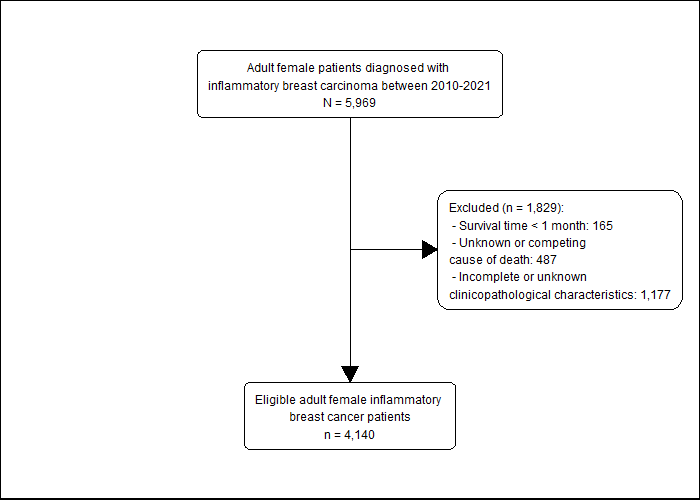
\includegraphics[width=0.9\textwidth,height=0.7\textheight]{../../results/figures/flowchart.png}

}

\caption{\label{fig-flowchart}{Flowchart of IBC patients screening on
SEER database}}

\end{figure}%

The clinicopathological characteristics of eligible patients are
summarized in Table~\ref{tbl-table1}. The age subgroup of 20--49 years
accounts for 35.1\% of Luminal B cases, a higher proportion compared to
other subtypes. Moreover, Luminal B and HER2-positive subtypes appear to
affect younger age groups more frequently than Luminal A, with 85.4\%
and 84.5\% of cases, respectively, occurring in patients under 69 years,
compared to 76.5\% for Luminal A. A higher proportion of Black patients
is observed in the Triple-Negative group compared to other subtypes.
Marital status analysis shows that the Triple-Negative group has the
highest percentage of unmarried women. Triple-Negative cases also have
the highest percentage of N3 node stage and exhibit the greatest
proportion of grade III/IV cases.

\begin{table}

\caption{\label{tbl-table1}{Clinicopathological characteristics by
cancer subtype}}

\centering{

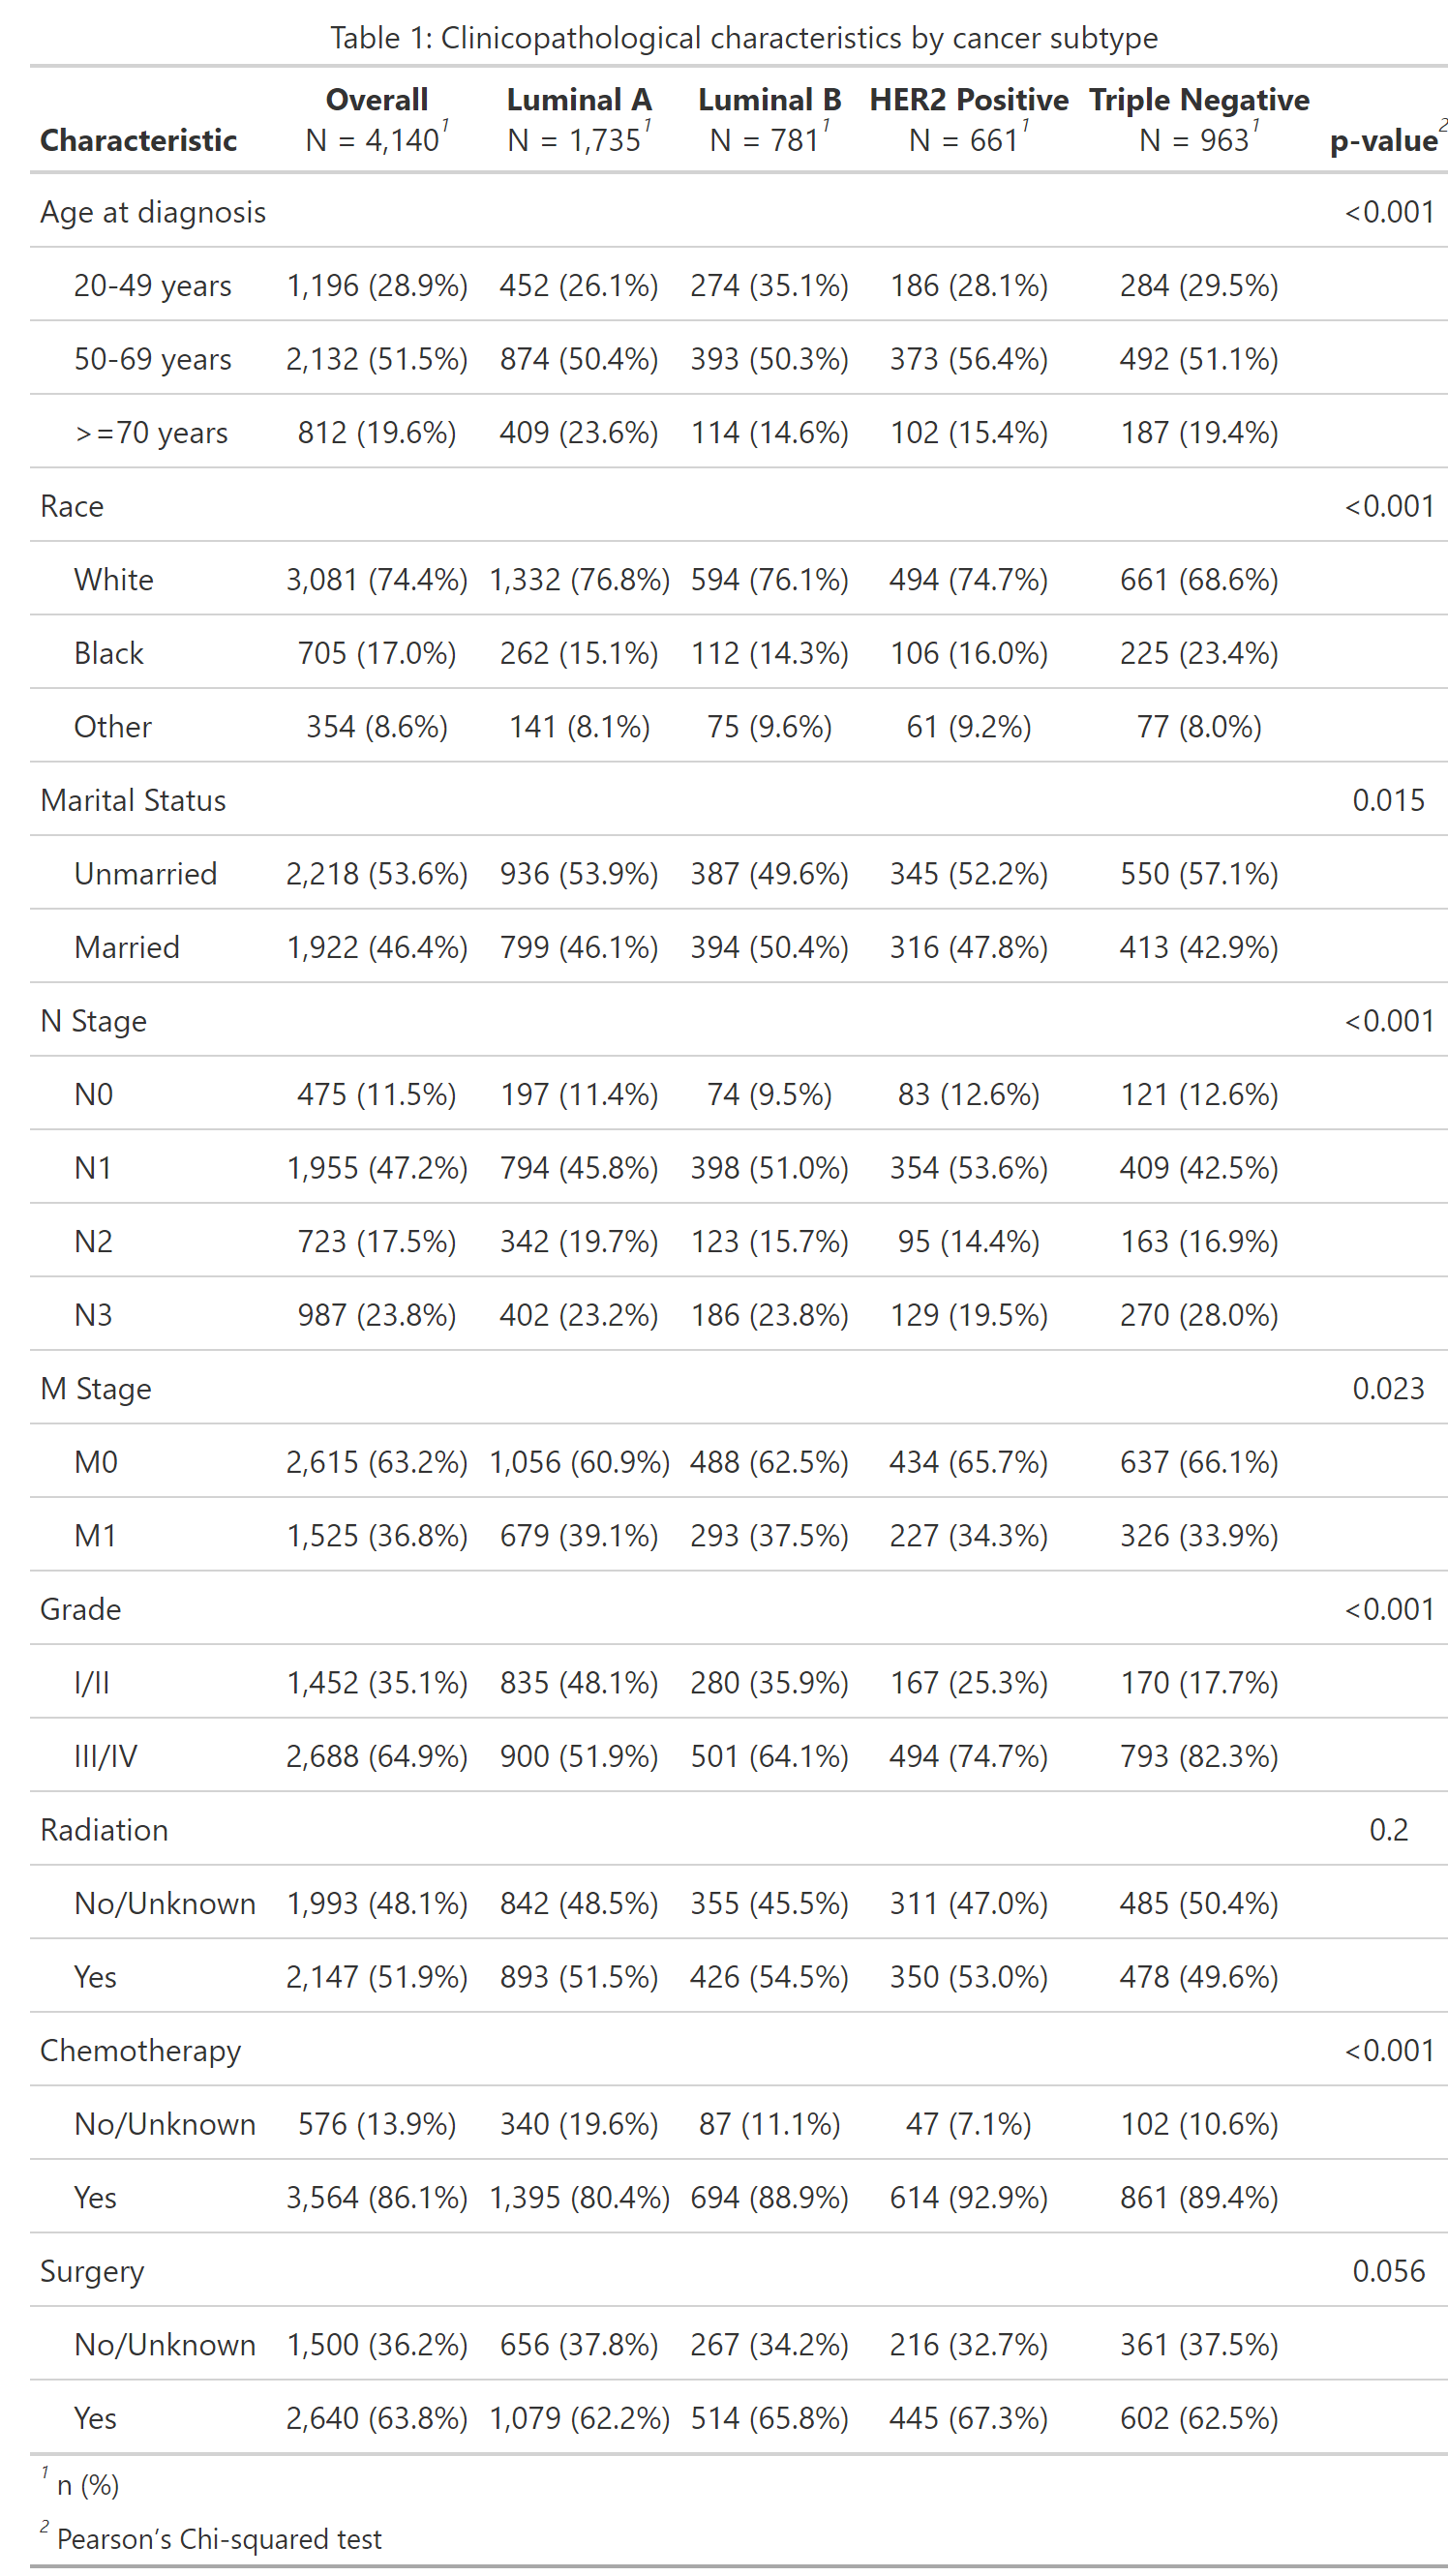
\includegraphics{../../results/tables/t1.rds}

}

\end{table}%

\clearpage

\subsection{Proportional Hazards
Assumption}\label{proportional-hazards-assumption}

The proportional hazards assumption was assessed for each covariate
visually using log minus log plots, as shown in Figure~\ref{fig-loglog}.

\begin{figure}

\centering{

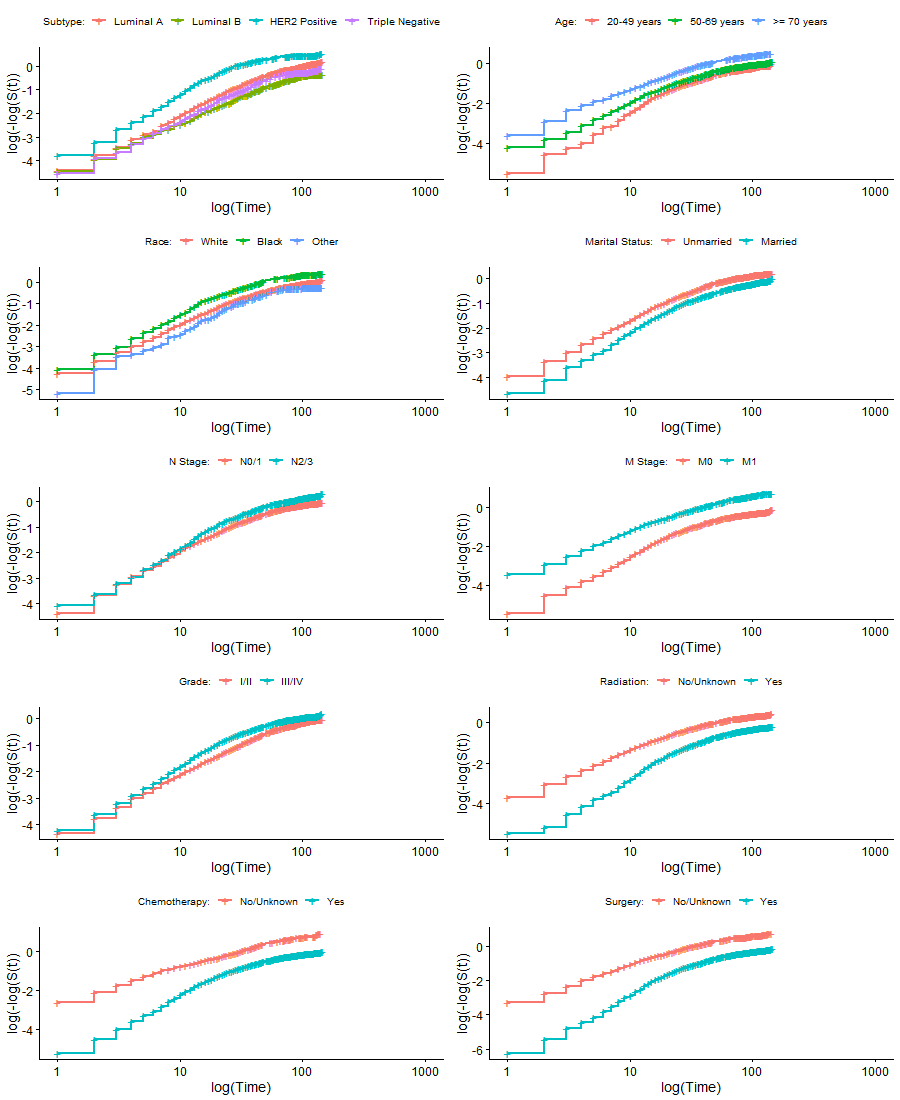
\includegraphics[width=1\textwidth,height=\textheight]{../../results/figures/loglog_plot.png}

}

\caption{\label{fig-loglog}{Log minus log plots}}

\end{figure}%

Upon inspection, slight deviations from parallelism were observed for
the covariates subtype, grade radiation, chemotherapy, and surgery.
Therefore, the full Cox proportional hazards model was fitted to the
data, and Schoenfeld residuals were extracted. The correlation between
Schoenfeld residuals and ranked survival times for each covariate is
presented in Table~\ref{tbl-table2}.

\begin{table}

\caption{\label{tbl-table2}{Schoenfeld Residual and Ranked Survival Time
Correlation}}

\centering{

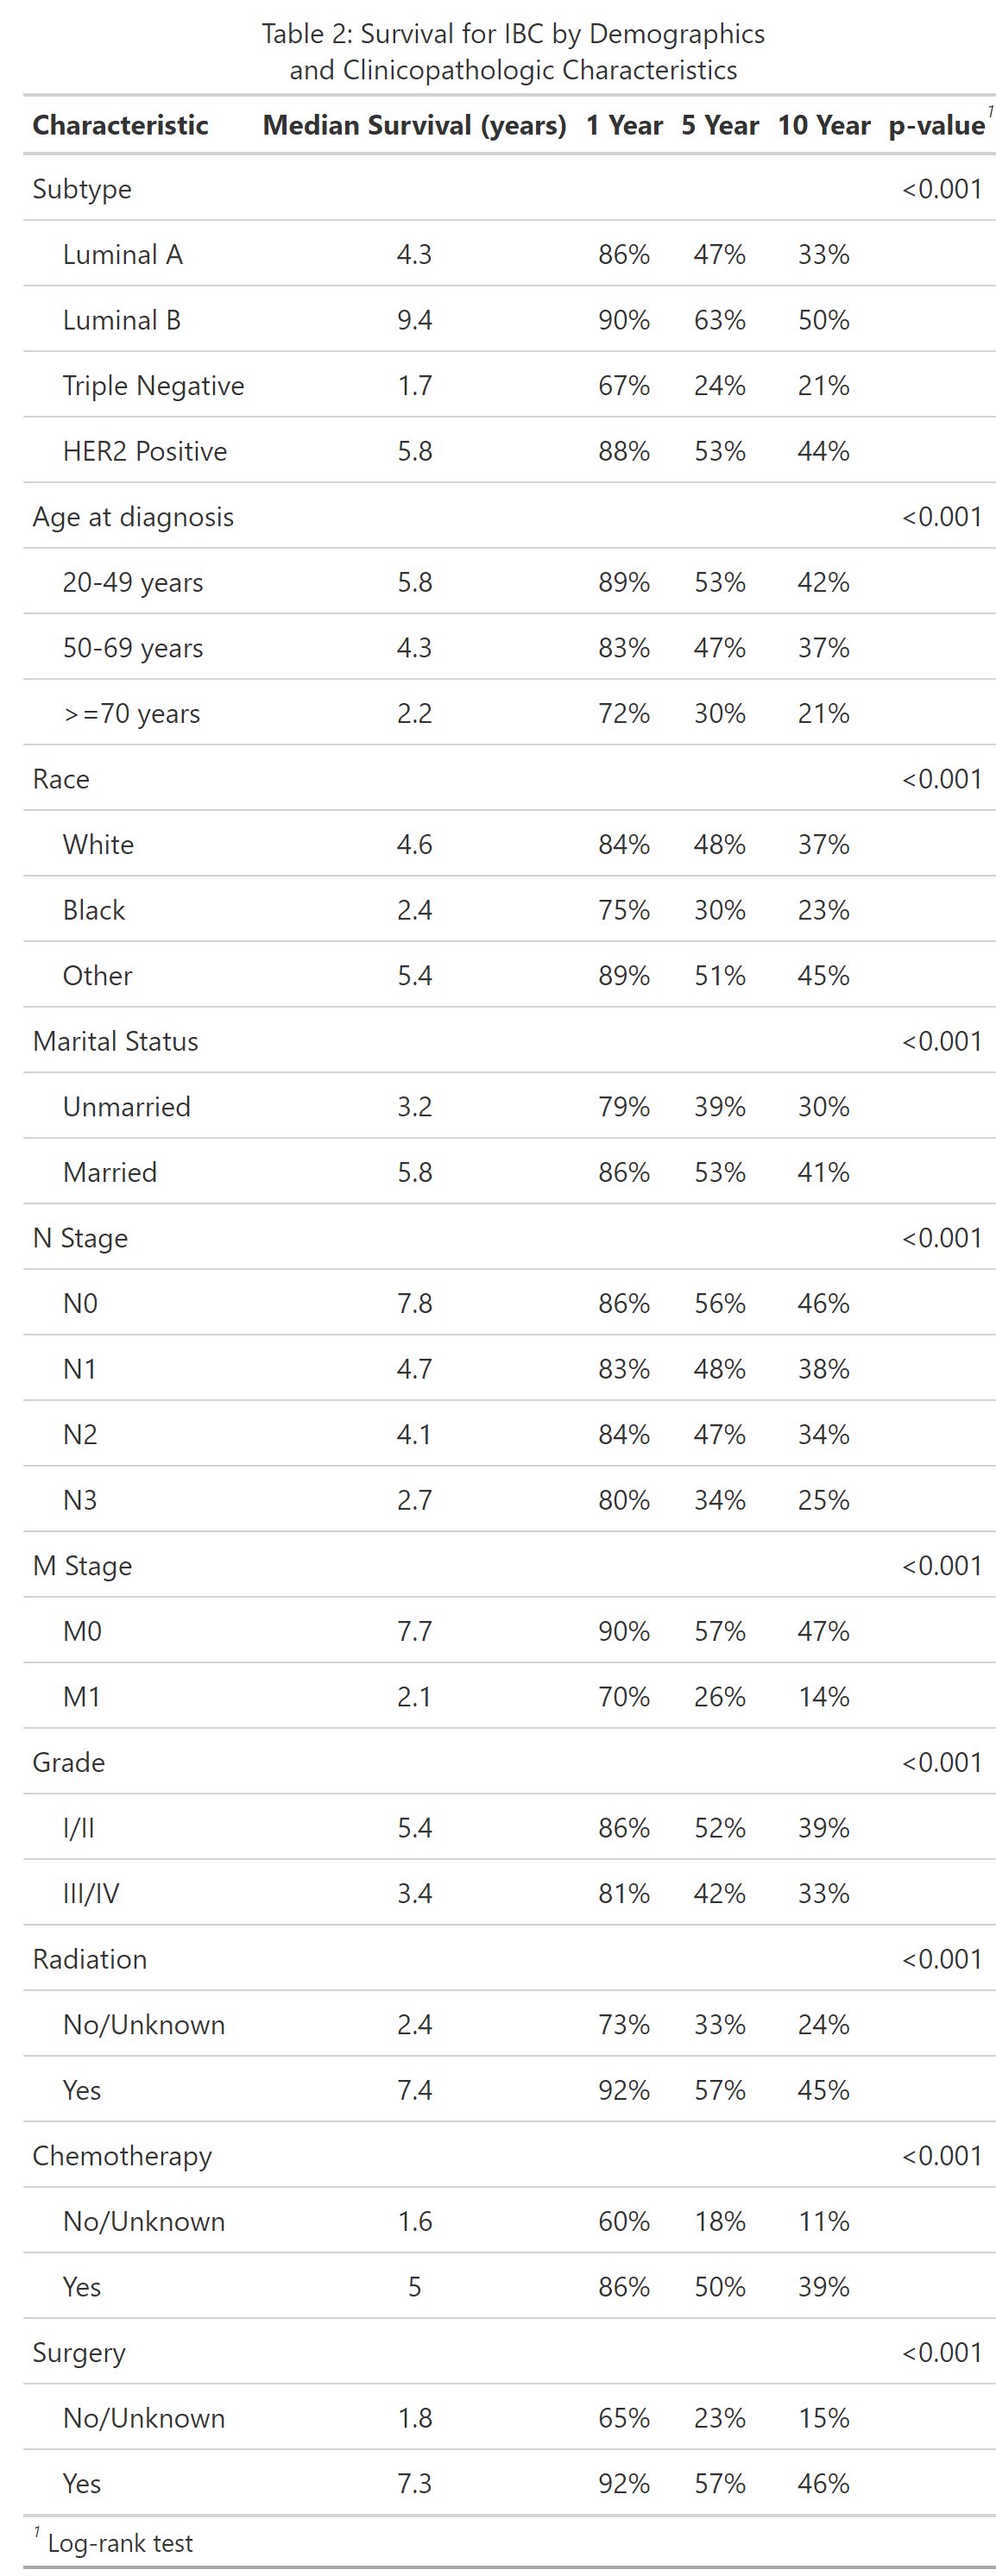
\includegraphics[width=0.4\textwidth,height=\textheight]{../../results/tables/t2.png}

}

\end{table}%

While the p-values for the covariates triple negative subtype, grade,
radiation, chemotherapy, and surgery are statistically significant at
the 0.05 level, the observed correlations are not of large magnitude.
Specifically, the correlations are -0.128, -0.042, 0.070, 0.110, and
0.074, respectively. Given that these values are relatively small in
magnitude, we proceed with the Cox proportional hazards regression
model.

\clearpage

\subsection{Survival Analysis}\label{survival-analysis}

Table~\ref{tbl-table3} presents the median survival in years, along with
1-, 5-, and 10-year survival percentages, stratified by
clinicopathological characteristics, all of which show statistically
significant differences based on the log-rank test. Survival outcomes
differ significantly by subtype, with the Triple-Negative subtype
showing the poorest prognosis, including a median survival of 1.7 years
and 1-, 5-, and 10-year survival rates of 67\%, 24\%, and 21\%,
respectively. Conversely, the Luminal B subtype has the most favorable
outcomes, with a median survival of 9.4 years and a 10-year survival
rate of 50\%. Racial disparities are evident, as Black patients have the
poorest survival outcomes, with a median survival of 2.4 years compared
to 4.6 years for White patients and 5.4 years for patients of other
races. Unmarried women experience poorer survival compared to married
women. Although 1-year survival is similar across all node stages, nodal
involvement significantly affects long-term outcomes, with the N3 stage
showing the lowest median survival of 2.7 years and the poorest 5- and
10-year survival rates. Survival differences are also pronounced by
distant metastasis (M stage), with M1 stage associated with worse
outcomes. Additionally, higher cancer grades correlate with poorer
survival. In terms of treatment, patients who receive radiation,
chemotherapy, or surgery exhibit better survival outcomes across all
measurements.

\begin{table}

\caption{\label{tbl-table3}{Survival for IBC by Clinicopathological
Characteristics}}

\centering{

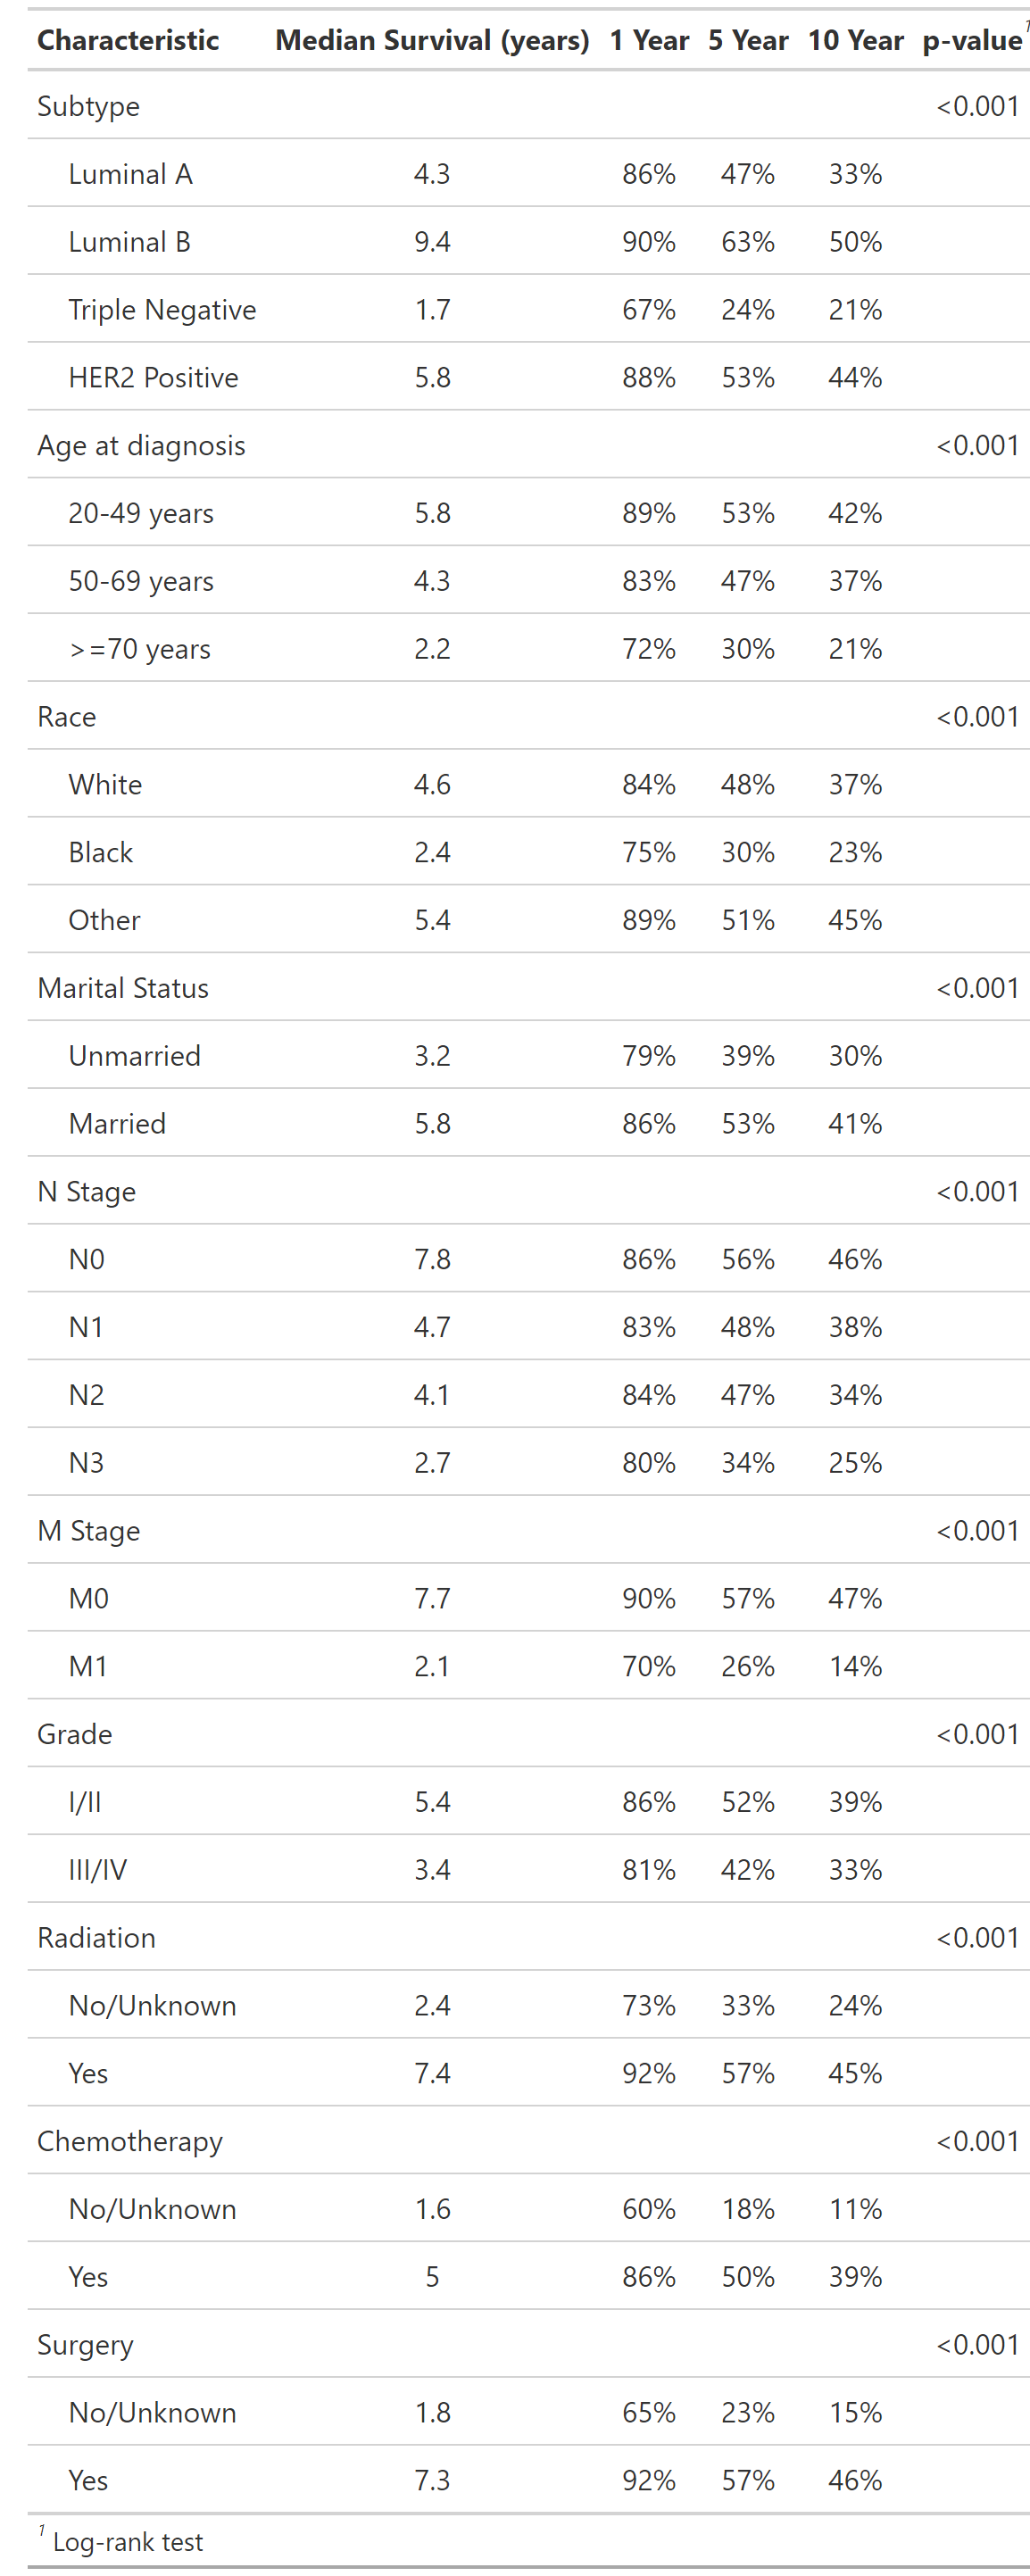
\includegraphics[width=1\textwidth,height=\textheight]{../../results/tables/t3.png}

}

\end{table}%

We conducted univariate and multivariate analyses based on the data in
Table~\ref{tbl-table3}, with the results of the Cox proportional hazards
regression presented in Table~\ref{tbl-table4}.

\begin{table}

\caption{\label{tbl-table4}{Cox Proportional Hazards Regression Model
for Survival in Adult Women with IBC}}

\centering{

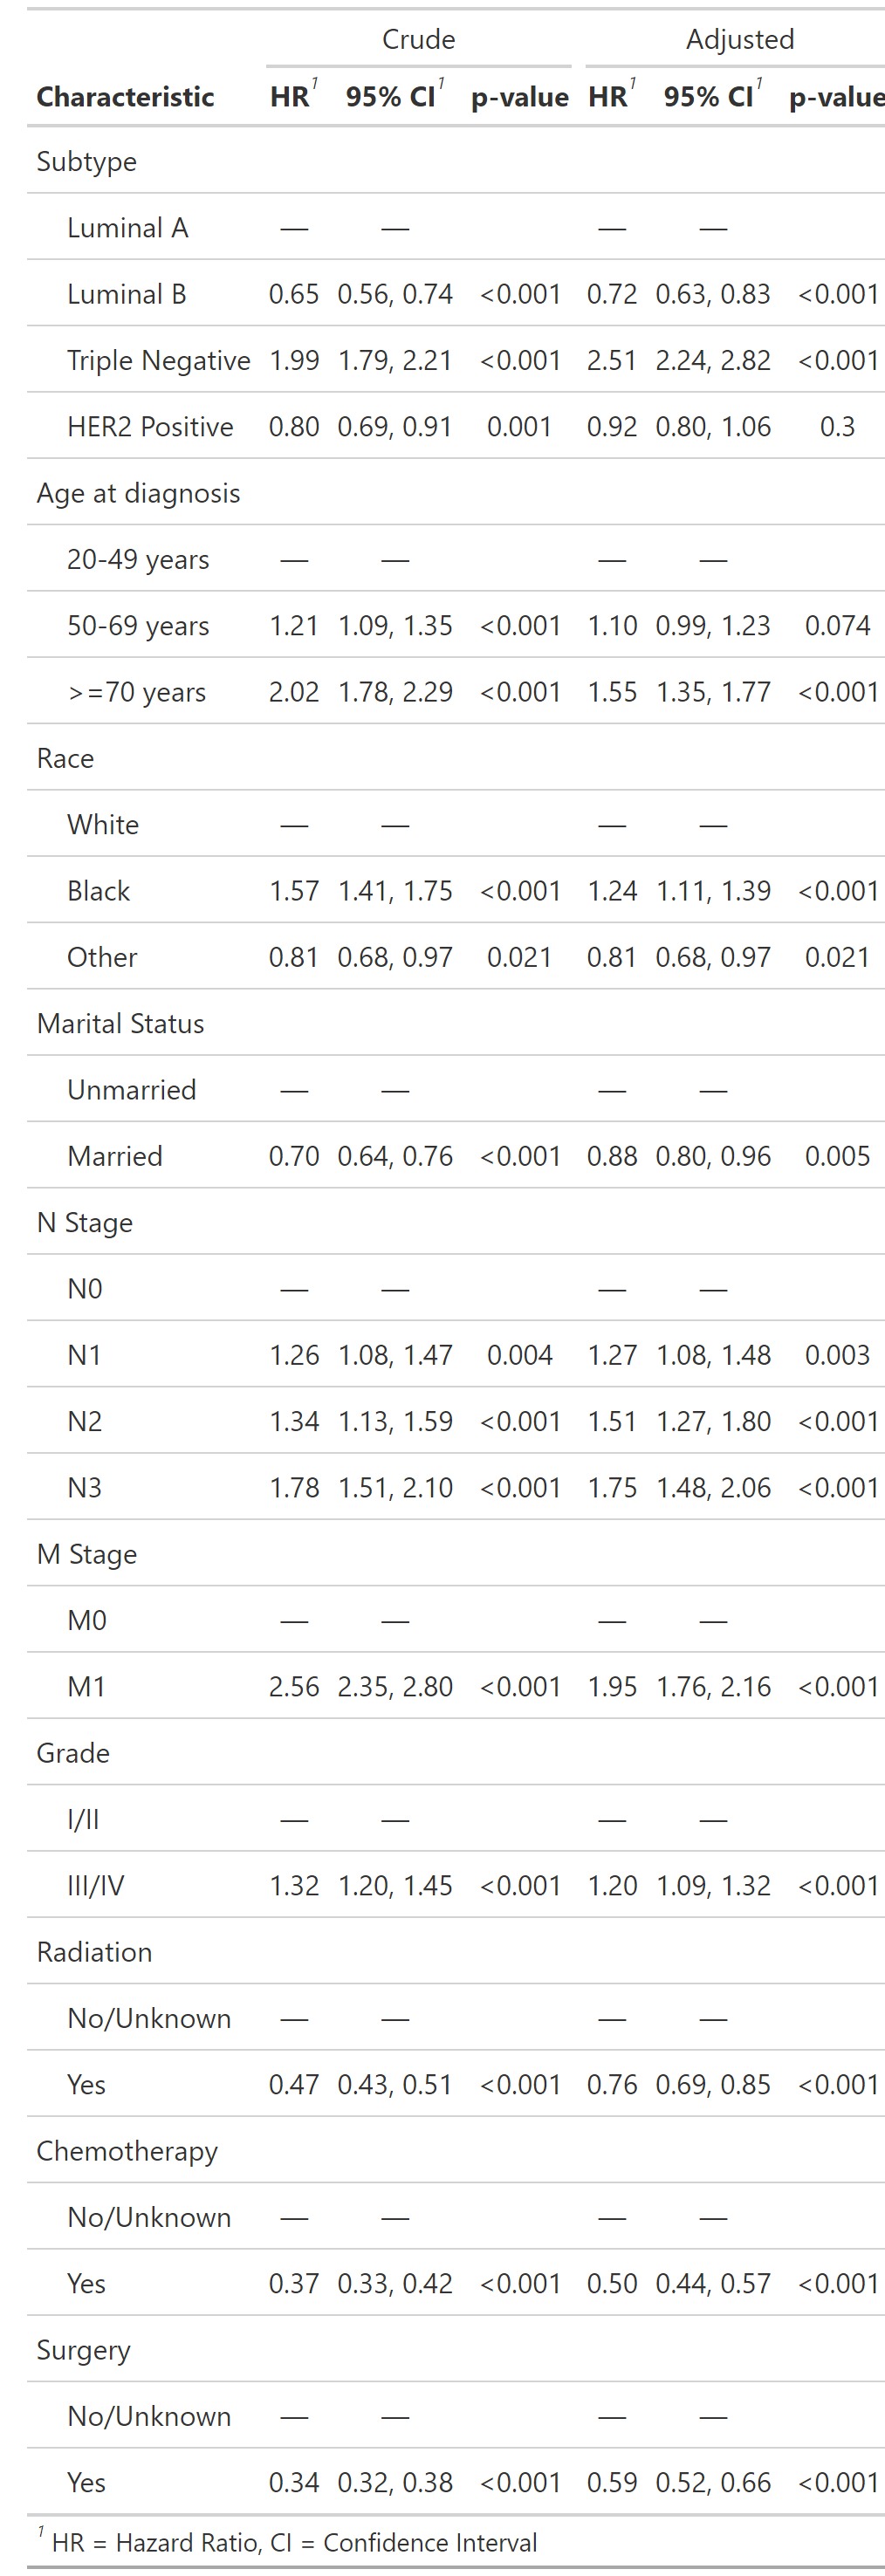
\includegraphics[width=1\textwidth,height=\textheight]{../../results/tables/t4.png}

}

\end{table}%

\subsection{Univariate Analysis}\label{univariate-analysis}

In the univariate analysis, subtype, age, race, marital status, N stage,
M stage, grade, radiation, chemotherapy, and surgery were all
significantly associated with IBC-specific survival. These variables
were therefore included in the multivariate analysis.

\subsection{Multivariate Analysis}\label{multivariate-analysis}

The multivariate analysis revealed that subtype, age, race, marital
status, N stage, M stage, grade, radiation, chemotherapy, and surgery
were independent predictors of IBC-specific survival. The Luminal B
subtype was associated with better survival (aHR=0.72, 95\%CI:
0.56-0.74, P\textless0.0001), whereas the Triple-Negative subtype showed
the poorest survival outcomes (aHR=2.51, 95\%CI: 1.79-2.21,
P\textless0.0001). In terms of treatment, our results find that the
existing therapies are effective in improving survival, that is
radiation (aHR=0.76, 95\%CI: 0.69-0.85, P\textless0.0001), chemotherapy
(aHR=0.50, 95\%CI: 0.44-0.57, P\textless0.0001), and surgery (aHR=0.59,
95\%CI: 0.52-0.66, P\textless0.0001).

\clearpage

\section{Discussion}\label{discussion}

In this large population-based cohort of women diagnosed with IBC, we
found a better survival in Luminal B molecular subtype and poorer in
Triple Negative. We found that Black patients made up the smallest
percentage of Luminal B subtype and the greatest of Triple Negative.
Similar findings were observed for patients who were unmarried at
diagnosis.

Take things that ive noted from other study and compare results here. It
would be interesting to look at the combination of treatments
(radiation, chemo, surgery) Also comparing subtype to broader range of
breat cancer not just IBC.

\phantomsection\label{refs}
\begin{CSLReferences}{1}{0}
\bibitem[\citeproctext]{ref-TCR28003}
Bonito, Maurizio Di, Monica Cantile, and Gerardo Botti. 2019.
{``Pathological and Molecular Characteristics of Inflammatory Breast
Cancer.''} \emph{Translational Cancer Research} 8 (Suppl 5).
\url{https://tcr.amegroups.org/article/view/28003}.

\bibitem[\citeproctext]{ref-devi2019perspectives}
Devi, Gayathri R, Holly Hough, Nadine Barrett, Massimo Cristofanilli,
Beth Overmoyer, Neil Spector, Naoto T Ueno, et al. 2019. {``Perspectives
on Inflammatory Breast Cancer (IBC) Research, Clinical Management and
Community Engagement from the Duke IBC Consortium.''} \emph{Journal of
Cancer} 10 (15): 3344.

\bibitem[\citeproctext]{ref-hance2005trends}
Hance, Kenneth W, William F Anderson, Susan S Devesa, Heather A Young,
and Paul H Levine. 2005. {``Trends in Inflammatory Breast Carcinoma
Incidence and Survival: The Surveillance, Epidemiology, and End Results
Program at the National Cancer Institute.''} \emph{Journal of the
National Cancer Institute} 97 (13): 966--75.

\bibitem[\citeproctext]{ref-iwamoto2011different}
Iwamoto, Takayuki, Giampaolo Bianchini, Yuan Qi, Massimo Cristofanilli,
Anthony Lucci, Wendy A Woodward, James M Reuben, et al. 2011.
{``Different Gene Expressions Are Associated with the Different
Molecular Subtypes of Inflammatory Breast Cancer.''} \emph{Breast Cancer
Research and Treatment} 125: 785--95.

\bibitem[\citeproctext]{ref-le2015future}
Le Du, Fanny, Bedrich L Eckhardt, Bora Lim, Jennifer K Litton, Stacy
Moulder, Funda Meric-Bernstam, Ana M Gonzalez-Angulo, and Naoto T Ueno.
2015. {``Is the Future of Personalized Therapy in Triple-Negative Breast
Cancer Based on Molecular Subtype?''} \emph{Oncotarget} 6 (15): 12890.

\bibitem[\citeproctext]{ref-li2017outcomes}
Li, Juanjuan, Yue Xia, Qi Wu, Shan Zhu, Chuang Chen, Wen Yang, Wen Wei,
and Shengrong Sun. 2017. {``Outcomes of Patients with Inflammatory
Breast Cancer by Hormone Receptor-and HER2-Defined Molecular Subtypes: A
Population-Based Study from the SEER Program.''} \emph{Oncotarget} 8
(30): 49370.

\bibitem[\citeproctext]{ref-menta2018inflammatory}
Menta, Arjun, Tamer M Fouad, Anthony Lucci, Huong Le-Petross, Michael C
Stauder, Wendy A Woodward, Naoto T Ueno, and Bora Lim. 2018.
{``Inflammatory Breast Cancer: What to Know about This Unique,
Aggressive Breast Cancer.''} \emph{Surgical Clinics} 98 (4): 787--800.

\bibitem[\citeproctext]{ref-robertson2010inflammatory}
Robertson, Fredika M, Melissa Bondy, Wei Yang, Hideko Yamauchi, Shannon
Wiggins, Samira Kamrudin, Savitri Krishnamurthy, et al. 2010.
{``Inflammatory Breast Cancer: The Disease, the Biology, the
Treatment.''} \emph{CA: A Cancer Journal for Clinicians} 60 (6):
351--75.

\bibitem[\citeproctext]{ref-tolaney2015adjuvant}
Tolaney, Sara M, William T Barry, Chau T Dang, Denise A Yardley, Beverly
Moy, P Kelly Marcom, Kathy S Albain, et al. 2015. {``Adjuvant Paclitaxel
and Trastuzumab for Node-Negative, HER2-Positive Breast Cancer.''}
\emph{New England Journal of Medicine} 372 (2): 134--41.

\end{CSLReferences}




\end{document}
